\section{半正定松弛}
\label{sec:cone-relax}

第~\ref{sec:cone-nonconvex-qp}小节的问题不能等价地改写成凸问题，KKT条件也给不出全局证书。既然改不成凸问题，能否算出一个有保证的下界，用它判断手上的候选解离最优还有多远？

\paragraph{把乘积收集到矩阵里}
考虑\term{二次约束二次规划}（quadratically constrained quadratic program，QCQP）
\begin{equation}
 \begin{aligned}
 \min_{\bm{x}\in\mathbb{R}^n}\quad&\bm{x}^\top\bm{Q}_0\bm{x}+2\bm{q}_0^\top\bm{x}+c_0\\
 \text{s.t.}\quad&\bm{x}^\top\bm{Q}_i\bm{x}+2\bm{q}_i^\top\bm{x}+c_i\leq0,\quad i=1,\ldots,m,
 \end{aligned}
 \label{eq:cone-qcqp}
\end{equation}
其中$\bm{Q}_i$对称，可以不定。等式约束可以拆成两条不等式，因此这里只写不等式。

难点全在乘积$x_ix_j$上。这些乘积在$\bm{x}$上是非线性的，但只要把它们看成新的未知数，每个二次式都变成新未知数的线性函数。这就像把一笔难算的账换一种记法：先不管各项之间的关系，只把用到的项登记下来，账立刻变成加法。这个类比的边界是：各项之间的关系并没有消失，它们藏在下面矩阵的结构里，后面要单独处理。

具体做法是引入带常数坐标的矩阵
\begin{equation}
 \bm{Y}=\begin{bmatrix}1\\\bm{x}\end{bmatrix}\begin{bmatrix}1\\\bm{x}\end{bmatrix}^\top=\begin{bmatrix}1&\bm{x}^\top\\\bm{x}&\bm{x}\bm{x}^\top\end{bmatrix}\in\mathcal{S}^{n+1},
 \label{eq:cone-lift-matrix}
\end{equation}
行列下标从$0$开始。常数坐标的作用是把线性项和常数项也放进矩阵。记
\[
 \bm{M}_i=\begin{bmatrix}c_i&\bm{q}_i^\top\\\bm{q}_i&\bm{Q}_i\end{bmatrix},
\]
直接展开迹内积，得到
\begin{equation}
 \bm{x}^\top\bm{Q}_i\bm{x}+2\bm{q}_i^\top\bm{x}+c_i=\langle\bm{M}_i,\bm{Y}\rangle.
 \label{eq:cone-lift-linear}
\end{equation}
原来的二次式成了$\bm{Y}$的线性函数。

图~\ref{fig:cone-lift}以式~\eqref{eq:cone-nonconvex-objective}为例。这时$\bm{Q}_0=\operatorname{diag}(1/2,-1/2)$，$\bm{q}_0=(0,1/8)$，$c_0=0$。

\begin{BookInlineFigure}
  \centering
  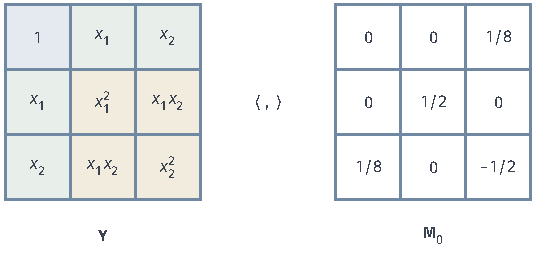
\includegraphics[width=90mm]{figures/05-optimization/06-constrained-optimization/tikz/cone-lift/figure.pdf}
  \caption{提升矩阵与目标系数。左边是$n=2$时的$\bm{Y}$，浅蓝格是常数，绿格是一次项，黄格是二次项。右边是目标$\frac12x_1^2-\frac12x_2^2+\frac14x_2$对应的$\bm{M}_0$，交叉项的系数对半分在两个对称位置上。二者的迹内积就是目标。}
  \label{fig:cone-lift}
\end{BookInlineFigure}

\paragraph{哪些矩阵来自向量}
不是每个矩阵都有式~\eqref{eq:cone-lift-matrix}的形状。下面的引理精确地指出需要哪些条件。

\begin{lemma}[秩一刻画]
\label{lem:cone-rank-one}
$\bm{Y}\in\mathcal{S}^{n+1}$具有式~\eqref{eq:cone-lift-matrix}的形状，当且仅当
\begin{equation}
 \bm{Y}\succeq\bm{0},\qquad Y_{0,0}=1,\qquad\operatorname{rank}\bm{Y}=1.
 \label{eq:cone-rank-one}
\end{equation}
\end{lemma}

\begin{proof}
式~\eqref{eq:cone-lift-matrix}的矩阵满足这三条：它是一个向量与自身的外积，秩为一且半正定，第一个元素是$1$。反过来，秩一半正定矩阵可以写成$\bm{Y}=\bm{v}\bm{v}^\top$。由$Y_{0,0}=v_0^2=1$得$v_0=\pm1$，必要时把$\bm{v}$换成$-\bm{v}$，可设$v_0=1$。记$\bm{v}=(1,\bm{x})$，$\bm{Y}$就有所要的形状。
\end{proof}

于是问题~\eqref{eq:cone-qcqp}等价于在条件~\eqref{eq:cone-rank-one}和$\langle\bm{M}_i,\bm{Y}\rangle\leq0$下最小化$\langle\bm{M}_0,\bm{Y}\rangle$。目标和约束都是线性的，半正定和$Y_{0,0}=1$也是凸约束，全部困难集中在秩一这一条上。

把它删掉，就得到\term{半正定松弛}（semidefinite relaxation）
\begin{equation}
 \begin{aligned}
 \min_{\bm{Y}\in\mathcal{S}^{n+1}}\quad&\langle\bm{M}_0,\bm{Y}\rangle\\
 \text{s.t.}\quad&\langle\bm{M}_i,\bm{Y}\rangle\leq0,\quad i=1,\ldots,m,\\
 &Y_{0,0}=1,\quad\bm{Y}\succeq\bm{0}.
 \end{aligned}
 \label{eq:cone-sdr}
\end{equation}

\subsection{松弛下界}
\label{sec:cone-relax-bound}

删掉一个约束，最优值只会变小。这一小节要把这件事写准确，并弄清楚上面的几步各自改变了什么。

\begin{theorem}[松弛给出下界]
\label{thm:cone-sdr-bound}
记问题~\eqref{eq:cone-qcqp}的最优值为$f^\star$，问题~\eqref{eq:cone-sdr}的最优值为$p_{\mathrm{rel}}$。则
\begin{equation}
 p_{\mathrm{rel}}\leq f^\star.
 \label{eq:cone-sdr-bound}
\end{equation}
\end{theorem}

\begin{proof}
任取问题~\eqref{eq:cone-qcqp}的可行点$\bm{x}$，按式~\eqref{eq:cone-lift-matrix}构造$\bm{Y}$。由引理~\ref{lem:cone-rank-one}，$\bm{Y}\succeq\bm{0}$且$Y_{0,0}=1$。由式~\eqref{eq:cone-lift-linear}，$\langle\bm{M}_i,\bm{Y}\rangle\leq0$，且$\langle\bm{M}_0,\bm{Y}\rangle$等于原目标值。所以$\bm{Y}$对问题~\eqref{eq:cone-sdr}可行，$p_{\mathrm{rel}}$不超过原目标值。对所有可行$\bm{x}$取下确界，即得结论。
\end{proof}

这个结论只用到定义~\ref{def:cone-equivalent}的第一条。第二条在这里不成立，因为松弛问题的可行矩阵不一定对应任何$\bm{x}$。表~\ref{tab:cone-relax-steps}把三步分开。

\begin{BookInlineTable}
  \centering
  \begin{tabular}{lll}
    \toprule
    步骤 & 做了什么 & 与原问题的关系\\
    \midrule
    提升 & 用$\bm{Y}$表示乘积，保留秩一 & 等价\\
    放松秩约束 & 删去$\operatorname{rank}\bm{Y}=1$ & 可行集变大，得到下界\\
    求解松弛 & 数值计算SDP & 近似解，下界需验证\\
    \bottomrule
  \end{tabular}
  \caption{半正定松弛的三个步骤。只有第一步不改变问题。}
  \label{tab:cone-relax-steps}
\end{BookInlineTable}

\begin{example}[松弛证明全局最优]
\label{ex:cone-relax-nonconvex}
回到目标~\eqref{eq:cone-nonconvex-objective}。可行集$-1\leq x_2\leq1$写成二次约束$x_2^2\leq1$。记$\bm{Y}$的元素
\[
 \bm{Y}=\begin{bmatrix}1&y_1&y_2\\y_1&X_{1,1}&X_{1,2}\\y_2&X_{1,2}&X_{2,2}\end{bmatrix}.
\]
松弛问题是在$X_{2,2}\leq1$、$\bm{Y}\succeq\bm{0}$下最小化
\[
 \frac12X_{1,1}-\frac12X_{2,2}+\frac14y_2.
\]

下面逐项估计目标。半正定矩阵的对角元非负，所以$X_{1,1}\geq0$。约束给出$X_{2,2}\leq1$。再由$\{0,2\}$行列对应的$2\times2$主子式非负，$y_2^2\leq X_{2,2}\leq1$，所以$y_2\geq-1$。三项合起来，
\[
 \frac12X_{1,1}-\frac12X_{2,2}+\frac14y_2\geq0-\frac12-\frac14=-\frac34.
\]
这个下界由点A对应的秩一矩阵取到，所以$p_{\mathrm{rel}}=-3/4$，也就是$f^\star=-3/4$。KKT条件区分不开A和B，松弛却直接证明了A是全局最优，而B的目标值$-1/4$高于下界，不是全局最优。
\end{example}

\paragraph{符号变量}
下面这个问题里，松弛一般不紧。设$\bm{W}\in\mathcal{S}^n$，考虑
\begin{equation}
 \min_{\bm{x}}\ \bm{x}^\top\bm{W}\bm{x}\quad\text{s.t.}\quad x_i^2=1,\quad i=1,\ldots,n.
 \label{eq:cone-sign-problem}
\end{equation}
变量只能取$\pm1$，这是一个把点分到两侧的组合问题。约束$x_i^2=1$恰好是二次的，提升后成为对角线上的线性条件，一条也不丢。

这里没有线性项，$\bm{Y}$中的$\bm{x}$块可以去掉。设$\bm{Y}$可行，记其$\bm{x}$块为$\hat{\bm{x}}$，令$\bm{D}_{\pm}=\operatorname{diag}(1,-\bm{I})$。矩阵$\bm{D}_{\pm}\bm{Y}\bm{D}_{\pm}$也可行，目标不变，只是$\hat{\bm{x}}$变号。二者的平均仍可行，而$\bm{x}$块为零。所以只需保留右下块$\bm{X}=\bm{x}\bm{x}^\top$，松弛写成
\begin{equation}
 \min_{\bm{X}\in\mathcal{S}^n}\ \langle\bm{W},\bm{X}\rangle\quad\text{s.t.}\quad X_{i,i}=1,\quad i=1,\ldots,n,\quad\bm{X}\succeq\bm{0}.
 \label{eq:cone-sign-relax}
\end{equation}
取$\bm{A}_i=\bm{e}_i\bm{e}_i^\top$、$b_i=1$，由式~\eqref{eq:cone-sdp-dual}，它的对偶问题是
\begin{equation}
 \max_{\bm{y}\in\mathbb{R}^n}\ \sum_{i=1}^ny_i\quad\text{s.t.}\quad\bm{W}-\operatorname{diag}(\bm{y})\succeq\bm{0}.
 \label{eq:cone-sign-dual}
\end{equation}

先看$n=2$，$\bm{W}$的对角元为零、非对角元为$1$。松弛的可行矩阵是$\begin{bmatrix}1&a\\a&1\end{bmatrix}$，$a\in[-1,1]$，目标是$2a$。最优在$a=-1$取到，矩阵秩一，对应$\bm{x}=(1,-1)$，松弛是紧的。

再看三角形的例子。取$n=3$，
\[
 \bm{W}=\begin{bmatrix}0&1&1\\1&0&1\\1&1&0\end{bmatrix}.
\]
目标是$2(x_1x_2+x_1x_3+x_2x_3)$。枚举$8$个符号组合，全同时目标为$6$，其余都是两个相同、一个相反，目标为$-2$。所以$f^\star=-2$。

松弛问题中取
\[
 \hat{\bm{X}}=\begin{bmatrix}1&-1/2&-1/2\\-1/2&1&-1/2\\-1/2&-1/2&1\end{bmatrix}.
\]
它的特征值是$0,3/2,3/2$，半正定，对角元都是$1$，所以松弛可行。六个非对角元各贡献$-1/2$，目标是
\[
 \langle\bm{W},\hat{\bm{X}}\rangle=-3.
\]

再看对偶问题~\eqref{eq:cone-sign-dual}。取$\bm{y}=(-1,-1,-1)$，则
\[
 \bm{W}-\operatorname{diag}(\bm{y})=\bm{W}+\bm{I}=\bm{1}\bm{1}^\top\succeq\bm{0},
\]
对偶目标是$-3$。原始和对偶的值相等，所以$p_{\mathrm{rel}}=-3$。

下界$-3$比真实最优值$-2$低了$1$，这个间隙来自放松秩约束，而不是求解误差。图~\ref{fig:cone-relax-slice}在切片上画出了可行集究竟扩大了多少。

\begin{BookInlineFigure}
  \centering
  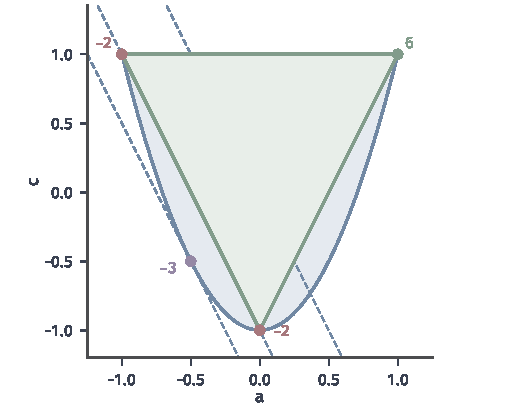
\includegraphics[width=88mm]{figures/05-optimization/06-constrained-optimization/matplotlib/cone-relax-slice/figure.pdf}
  \caption{$n=3$时松弛可行集在切片$X_{1,2}=X_{1,3}=a$、$X_{2,3}=c$上的形状。浅蓝抛物线区域$2a^2-1\leq c\leq1$是松弛的可行集。绿色三角形是秩一矩阵（符号解）的凸包，其顶点旁标注目标$4a+2c$的值。蓝色虚线是等值线，紫点是松弛最优解，目标$-3$，它在三角形之外。}
  \label{fig:cone-relax-slice}
\end{BookInlineFigure}

切片的形状可以直接算出来。矩阵$\begin{bmatrix}1&a&a\\a&1&c\\a&c&1\end{bmatrix}$有特征向量$(0,1,-1)$，特征值$1-c$，要求$c\leq1$。在与之正交的子空间上，矩阵约化为$\begin{bmatrix}1&\sqrt2a\\\sqrt2a&1+c\end{bmatrix}$，半正定要求$1+c\geq2a^2$。

\subsection{原解恢复}
\label{sec:cone-relax-recovery}

松弛的解是矩阵，原问题要的是向量。这一小节回答：什么时候可以把向量直接读出来，读不出来时又该怎么办？

\paragraph{秩一的情形}
若松弛的最优矩阵恰好秩一，问题就结束了。

\begin{theorem}[秩一解恢复原问题的最优解]
\label{thm:cone-rank-one-exact}
设$\bm{Y}^\star$是问题~\eqref{eq:cone-sdr}的最优解，且$\operatorname{rank}\bm{Y}^\star=1$。取$\bm{x}^\star$为$\bm{Y}^\star$第$0$列的后$n$个元素。则$\bm{x}^\star$是问题~\eqref{eq:cone-qcqp}的全局最优解，且$p_{\mathrm{rel}}=f^\star$。
\end{theorem}

\begin{proof}
由引理~\ref{lem:cone-rank-one}，$\bm{Y}^\star$具有式~\eqref{eq:cone-lift-matrix}的形状，其中的向量就是$\bm{x}^\star$。由式~\eqref{eq:cone-lift-linear}，$\bm{x}^\star$满足全部约束，目标值等于$p_{\mathrm{rel}}$。结合式~\eqref{eq:cone-sdr-bound}，
\[
 f(\bm{x}^\star)=p_{\mathrm{rel}}\leq f^\star\leq f(\bm{x}^\star).
\]
所以三者相等。
\end{proof}

定理依赖于约束的对应关系：松弛必须把原问题的每条约束都按式~\eqref{eq:cone-lift-linear}写了进去。若为了省事删掉了某条约束，恢复的$\bm{x}^\star$还要单独检查这条约束。

\paragraph{高秩的情形}
矩阵的秩大于$1$时，它不是任何向量的外积，松弛的最优矩阵不是原问题的可行解。这时要把矩阵“变回”向量，常用两种办法：取最大特征值对应的特征向量作投影；或者把矩阵分解后随机取整。无论哪一种，都是问题专属的启发式步骤。

对符号问题，常用的取整步骤如下\scite{goemans1995maxcut}。把$\bm{X}$分解成$X_{i,j}=\bm{v}_i^\top\bm{v}_j$，$\bm{v}_i$是单位向量，因为对角元是$1$。随机抽取一个标准高斯向量$\bm{g}$，令
\begin{equation}
 x_i=\operatorname{sign}(\bm{v}_i^\top\bm{g}).
 \label{eq:cone-rounding}
\end{equation}
几何上，这是用一个随机的超平面把各个单位向量分成两侧，同侧的$x_i$相同。

两个向量被分开的概率与它们的夹角成正比。$\bm{g}$在$\bm{v}_i,\bm{v}_j$所在平面上的投影方向是均匀的，夹角为$\theta$时被分开的概率是$\theta/\pi$。于是
\begin{equation}
 \mathbb{E}[x_ix_j]=1-\frac{2\theta}{\pi}=\frac{2}{\pi}\arcsin X_{i,j}.
 \label{eq:cone-rounding-expectation}
\end{equation}
最后一步用了$\theta=\arccos X_{i,j}$和$\arcsin z=\pi/2-\arccos z$。

三角形的$\hat{\bm{X}}$可以分解成平面上三个互成$120^\circ$的单位向量，见图~\ref{fig:cone-round-vectors}(a)。任何一条过原点的直线都把三个向量分成一个和两个。所以取整结果总是两同一异，目标总是$-2$，碰巧等于$f^\star$。由式~\eqref{eq:cone-rounding-expectation}验证，$\mathbb{E}[x_ix_j]=-1/3$，目标的期望是$6\cdot(-1/3)=-2$。

\begin{BookInlineFigure}
  \centering
  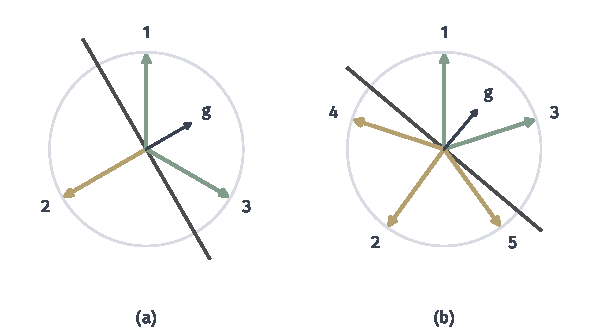
\includegraphics[width=100mm]{figures/05-optimization/06-constrained-optimization/matplotlib/cone-round-vectors/figure.pdf}
  \caption{随机超平面取整。深灰线是与随机方向$\bm{g}$垂直的直线，绿色向量对应$x_i=1$，黄色向量对应$x_i=-1$。(a)三角形问题的三个向量互成$120^\circ$。(b)五边形问题的五个向量，相邻编号之间夹角$144^\circ$。}
  \label{fig:cone-round-vectors}
\end{BookInlineFigure}

\paragraph{恢复可能破坏可行性}
取整会改变目标，也会破坏约束。设问题~\eqref{eq:cone-sign-problem}中$n=4$，再加上平衡约束$x_1+x_2+x_3+x_4=0$。把它平方后提升为$\langle\bm{1}\bm{1}^\top,\bm{X}\rangle=0$。矩阵
\[
 \bm{X}=\frac43\bm{I}-\frac13\bm{1}\bm{1}^\top
\]
对角元为$1$，非对角元为$-1/3$，特征值是$4/3,4/3,4/3,0$，且$\langle\bm{1}\bm{1}^\top,\bm{X}\rangle=4-12/3=0$，满足松弛的全部约束。

它对应四面体的四个顶点方向，这四个向量和为零，一个超平面不可能把它们全放在同一侧，取整结果只有两种：二比二（满足平衡约束）或一比三（$(\sum_ix_i)^2=4$，违反约束）。由式~\eqref{eq:cone-rounding-expectation}，
\[
 \mathbb{E}\Bigl[\bigl(\sum_ix_i\bigr)^2\Bigr]=4+12\cdot\frac2\pi\arcsin\Bigl(-\frac13\Bigr)\approx1.404.
\]
除以$4$，一比三的概率约为$0.351$。超过三分之一的取整结果是不可行的，必须修复或丢弃后重新检验。

\subsection{上下界检验}
\label{sec:cone-relax-bounds}

松弛算出来的数字到底保证了什么？这一小节把上界、下界和间隙分别交代清楚。

\paragraph{两个界}
一个经过原约束核对的点$\hat{\bm{x}}$给出上界$U=f(\hat{\bm{x}})$。一个松弛的对偶可行解$\bm{y}$给出下界$L$，对符号问题就是$L=\sum_iy_i$。合起来是一条链：
\begin{equation}
 L\leq p_{\mathrm{rel}}\leq f^\star\leq U.
 \label{eq:cone-bound-chain}
\end{equation}
报告时写出$U-L$。它同时包含松弛自身的间隙和求解的误差，是对$\hat{\bm{x}}$质量的一个可靠估计。

在三角形例子中，$U=-2$，$L=-3$，$U-L=1$。这里$\hat{\bm{x}}$其实已经最优，间隙全部来自松弛，继续迭代也不会缩小。间隙不为零，不代表候选解不好。

\paragraph{近似原始值不是下界}
常见的错误是把松弛问题的一个可行矩阵的目标值当作下界。式~\eqref{eq:cone-bound-chain}中排在$f^\star$左边的是$p_{\mathrm{rel}}$，而可行矩阵$\hat{\bm{X}}$的目标值满足的是
\[
 \langle\bm{W},\hat{\bm{X}}\rangle\geq p_{\mathrm{rel}},
\]
方向相反。它可以高于$f^\star$。

取三角形问题中对角元为$1$、非对角元为$-0.3$的矩阵，特征值是$0.4,1.3,1.3$，松弛可行，目标是$-1.8$。可$f^\star=-2<-1.8$。若把$-1.8$当作下界，就会错误地断言符号问题的最优值不低于$-1.8$，如图~\ref{fig:cone-bounds-line}所示。

\begin{BookInlineFigure}
  \centering
  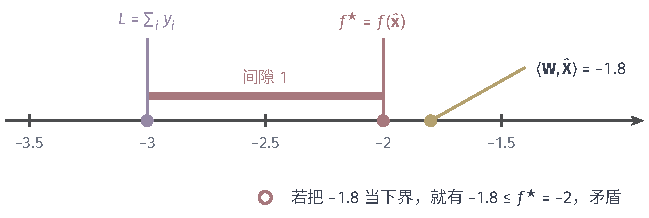
\includegraphics[width=110mm]{figures/05-optimization/06-constrained-optimization/tikz/cone-bounds-line/figure.pdf}
  \caption{三角形符号问题的各个数值。紫点是对偶可行解给出的下界$L=-3$，红点是最优值$f^\star=-2$，它也等于取整解的上界。黄点是松弛的一个未收敛可行矩阵的目标值$-1.8$，位于$f^\star$右侧，不能当作下界。红色粗线是报告的间隙。}
  \label{fig:cone-bounds-line}
\end{BookInlineFigure}

\paragraph{从近似对偶解得到有效下界}
数值求解器返回的$\bm{y}$往往只是近似可行，$\bm{W}-\operatorname{diag}(\bm{y})$可能有微小的负特征值，严格说来式~\eqref{eq:cone-bound-chain}不能用。幸好符号问题的对偶可行性很容易修复。

\begin{lemma}[修复对偶可行性]
\label{lem:cone-repair-dual}
对任意$\bm{y}\in\mathbb{R}^n$，记$\lambda$为矩阵$\bm{W}-\operatorname{diag}(\bm{y})$的最小特征值。则
\begin{equation}
 L(\bm{y})=\sum_{i=1}^ny_i+n\lambda
 \label{eq:cone-repaired-bound}
\end{equation}
是问题~\eqref{eq:cone-sign-relax}的最优值的下界，因而也是$f^\star$的下界。
\end{lemma}

\begin{proof}
令$\bm{y}'=\bm{y}+\lambda\bm{1}$。则
\[
 \bm{W}-\operatorname{diag}(\bm{y}')=\bm{W}-\operatorname{diag}(\bm{y})-\lambda\bm{I}\succeq\bm{0},
\]
因为最小特征值被平移到了零。所以$\bm{y}'$是问题~\eqref{eq:cone-sign-dual}的可行解，目标是$\sum_iy_i+n\lambda$。由弱对偶和定理~\ref{thm:cone-sdr-bound}得到结论。
\end{proof}

这个界对任何$\bm{y}$都成立，只要算得出最小特征值。例如在三角形问题中取不可行的$\bm{y}=(-1.1,-0.9,-1)$，最小特征值约为$-0.059$，修复后$L\approx-3.177$，仍是有效的下界。数值计算特征值本身有误差，严格的报告还要再减去一个反映舍入误差的小量。

图~\ref{fig:cone-bounds-iter}是一个$10$个变量的符号问题，权重是固定种子生成的$\pm1$。枚举全部符号组合得到$f^\star=-46$。求解松弛时，绿线是原始可行矩阵的目标值，紫线是由式~\eqref{eq:cone-repaired-bound}修复的下界。

\begin{BookInlineFigure}
  \centering
  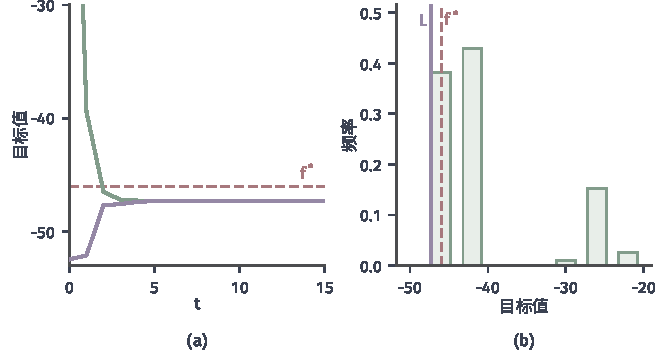
\includegraphics[width=112mm]{figures/05-optimization/06-constrained-optimization/matplotlib/cone-bounds-iter/figure.pdf}
  \caption{$n=10$的符号问题（$\bm{W}$的非对角元为随机$\pm1$，种子$7$）。(a)松弛的求解过程：绿线是可行矩阵的目标值，紫线是修复后的对偶下界，红色虚线是枚举得到的$f^\star=-46$。前两步绿线高于$f^\star$，不是$f^\star$的下界；收敛后二者相遇在$L\approx-47.28$。(b)从最终矩阵取整$2000$次得到的目标值分布，紫线是$L$，红色虚线是$f^\star$。}
  \label{fig:cone-bounds-iter}
\end{BookInlineFigure}

绿线在开始两步高于$f^\star$，把它当下界会得到错误的结论。收敛后两条线都停在$-47.28$附近，这就是$p_{\mathrm{rel}}$，它比$f^\star$低约$1.28$。这段距离是放松秩约束的代价，再多的迭代也消除不了。

图的(b)部分取整$2000$次。约$38\%$的试验得到$-46$，也就是真实最优值；其余的目标更差，最差到$-22$。所以取整要重复多次，取其中最好的可行点作为上界。这里$U=-46$，$U-L\approx1.28$，已经足以说明候选解很接近最优。

表~\ref{tab:cone-reported-quantities}整理了各个量的含义和要做的核对。

\begin{BookInlineTable}
  \centering
  \begin{tabular}{lll}
    \toprule
    量 & 保证 & 需要核对\\
    \midrule
    $f(\hat{\bm{x}})$ & $f^\star$的上界 & $\hat{\bm{x}}$满足原约束\\
    $\sum_iy_i$ & $f^\star$的下界 & $\bm{y}$对偶可行\\
    $\langle\bm{W},\hat{\bm{X}}\rangle$ & 收敛时接近$p_{\mathrm{rel}}$ & 不是$f^\star$的界\\
    $U-L$ & 候选解的最优性间隙 & 上下两界都已核对\\
    \bottomrule
  \end{tabular}
  \caption{半正定松弛的结果中各个量的含义。}
  \label{tab:cone-reported-quantities}
\end{BookInlineTable}
